% !TEX program = xelatex
% Compile with XeLaTeX (metropolis + Fira Sans) -- NOT pdflatex.
%   latexmk -xelatex slides.tex
\documentclass[10pt,aspectratio=169]{beamer}

\usetheme{metropolis}
\metroset{block=fill, progressbar=frametitle, sectionpage=progressbar, numbering=fraction}

\usepackage{appendixnumberbeamer}
\usepackage{booktabs}
\usepackage{pgfplots}
\pgfplotsset{compat=1.18}
\usetikzlibrary{arrows.meta, positioning}

% Restrained, cohesive teal/charcoal palette (no bright defaults).
\definecolor{accent}{HTML}{2A7F8E}
\setbeamercolor{alerted text}{fg=accent}
\setbeamercolor{progress bar}{fg=accent}
\setbeamercolor{frametitle}{bg=mDarkTeal}
% Unify example blocks into the same restrained palette (no default green).
\setbeamercolor{block title example}{use={block title}, fg=accent, bg=block title.bg}
\setbeamercolor{block body example}{use={block body}, bg=block body.bg}

\newcommand{\code}[1]{{\small\ttfamily #1}}
\tikzset{
  lp/.style={draw=accent, line width=0.6pt, rounded corners=2pt,
             inner sep=5pt, align=center, font=\small},
  fl/.style={-{Stealth[length=5pt]}, accent, line width=0.7pt},
}

\title{Diagnosing Small-Model Failures in MemGPT-Style Memory Retrieval}
\subtitle{Tool-Call Control, Query Policy, and Teacher-Trajectory Distillation}
\author{Hyogi Kim}
\institute{Ulsan National Institute of Science and Technology}
\date{}

\begin{document}

\maketitle

% ---------------------------------------------------------------
\begin{frame}{Memory has to outlive the context window}
  A persistent assistant must answer about things no longer in context:
  \begin{quote}
    \emph{``What artist did I say I could get into?''}
  \end{quote}
  \vspace{0.5em}
  The answer lives in a \alert{past session}---one specific earlier utterance,
  not world knowledge.
  \begin{quote}\small
    Speaker: \emph{``A little bit. I can get into Taylor Swift.''}
  \end{quote}
  \vspace{0.3em}
  The agent has to \alert{recover that utterance} and ground the answer in it.
\end{frame}

% ---------------------------------------------------------------
\begin{frame}{MemGPT: virtual memory for an LLM}
  \begin{center}
    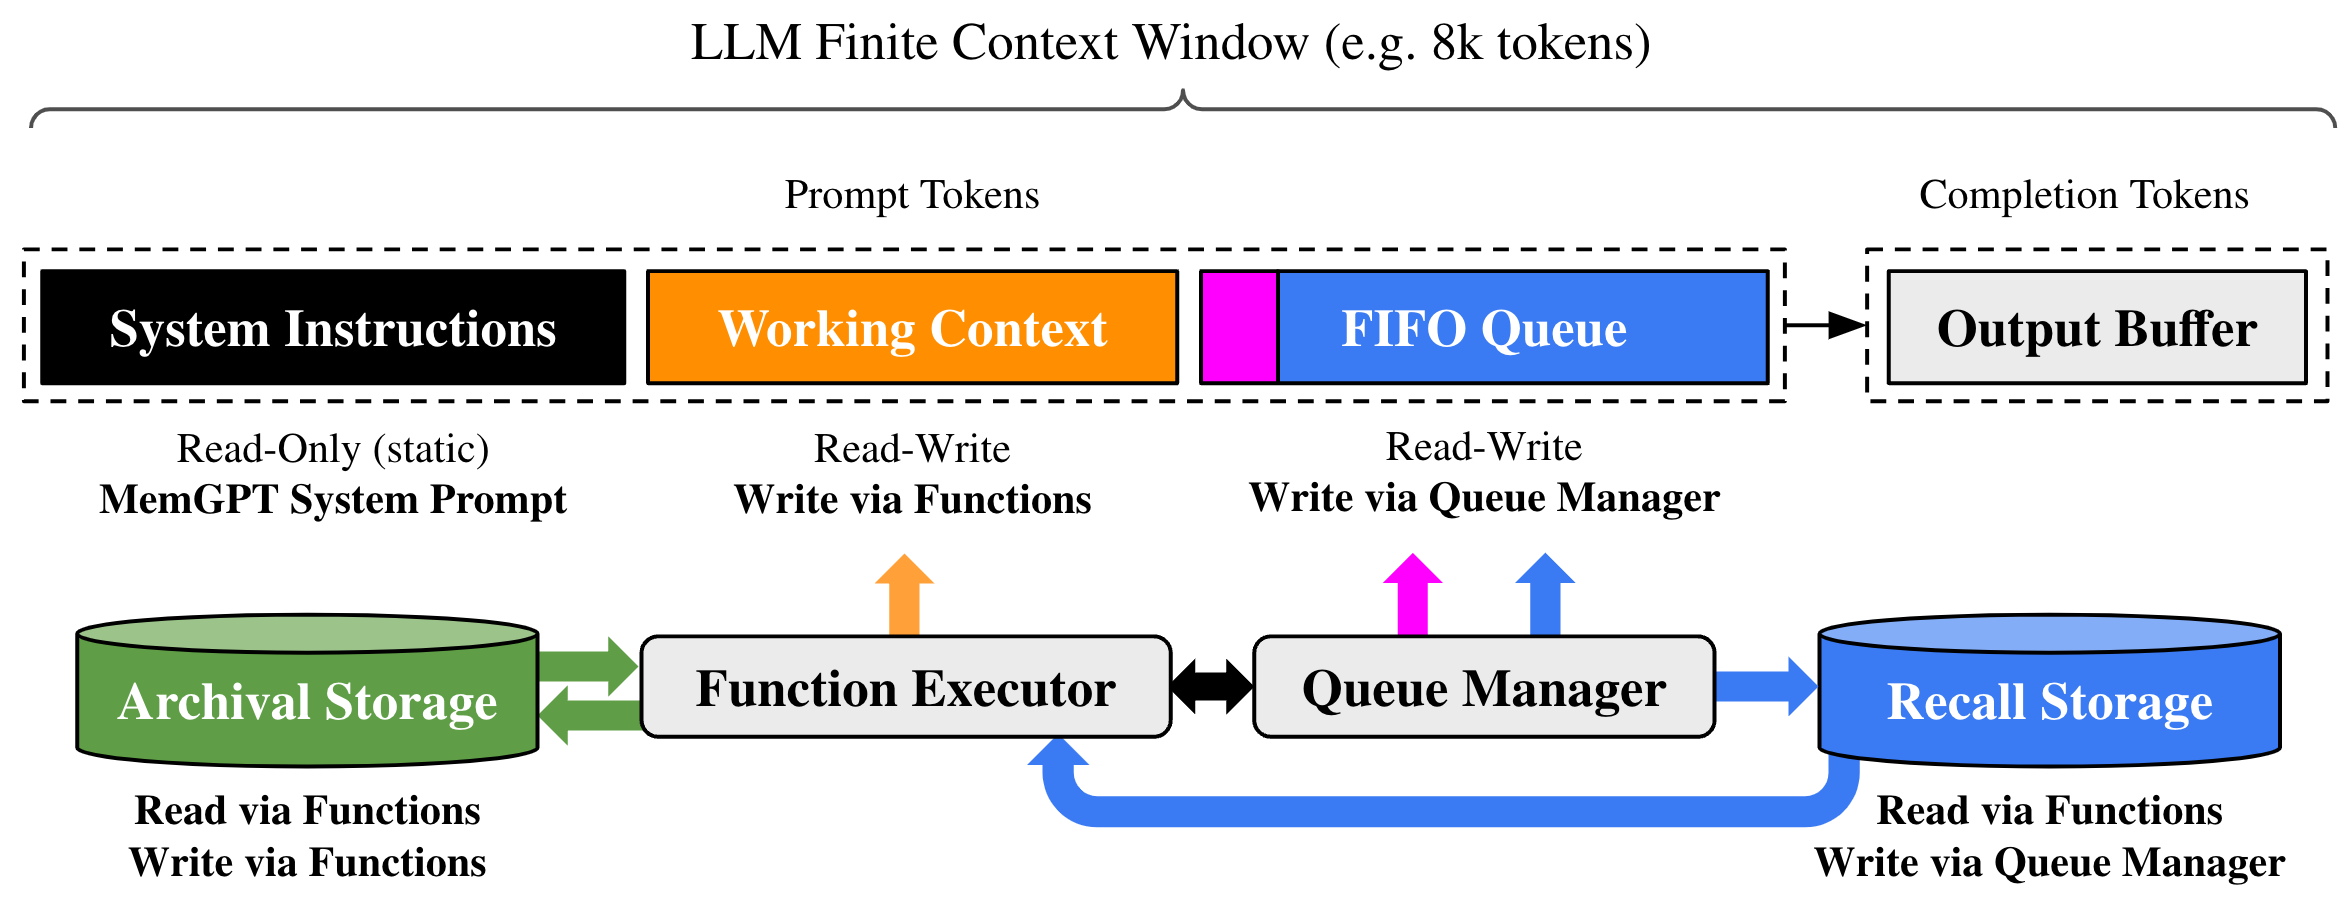
\includegraphics[width=0.70\textwidth]{MemGPT-diagram.png}
  \end{center}
  \vspace{0.3em}
  {\small The context window is small, tiered working memory; \alert{Archival}
  and \alert{Recall} storage are the large external memory, reached
  \alert{only through function calls}.}
  \par\vspace{0.3em}
  {\small In this work we use only the
  \alert{Recall\,/\,\texttt{conversation\_search}} path (not archival), and that
  recall is \alert{substring, not semantic}.}
  \par\vspace{0.3em}
  {\scriptsize Figure: Packer et al.\ (2023).}
\end{frame}

% ---------------------------------------------------------------
\begin{frame}{MemGPT makes recall a control problem}
  The model is a \alert{controller over memory tools}---it does not answer at once.
  \vspace{1.2em}
  \begin{center}
  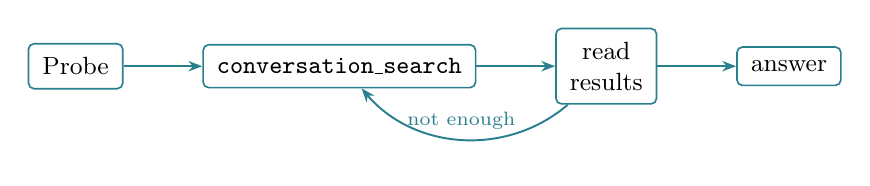
\begin{tikzpicture}[node distance=10mm]
    \node[lp] (p) {Probe};
    \node[lp, right=of p] (s) {\code{conversation\_search}};
    \node[lp, right=of s] (r) {read\\results};
    \node[lp, right=of r] (a) {answer};
    \draw[fl] (p) -- (s);
    \draw[fl] (s) -- (r);
    \draw[fl] (r) -- (a);
    \draw[fl] (r) to[bend left=45] node[above, font=\scriptsize, text=accent] {not enough} (s);
  \end{tikzpicture}
  \end{center}
  \vspace{1.0em}
  The hidden difficulty is not the answer---it is \alert{deciding how to operate
  the memory system}.
\end{frame}

% ---------------------------------------------------------------
\begin{frame}{One question behind a low score}
  When a small open model is weak at deep memory retrieval, is it because
  \vspace{1.2em}
  \begin{columns}[T,onlytextwidth]
    \column{0.46\textwidth}
      \begin{block}{Knowledge}
        it cannot form the answer\\ even \emph{with} the evidence?
      \end{block}
    \column{0.46\textwidth}
      \begin{block}{Behavior}
        it cannot \emph{operate} the\\ memory loop to get there?
      \end{block}
  \end{columns}
  \vspace{1.2em}
  We answer this by taking the loop apart, \alert{one component at a time}.
\end{frame}

% ---------------------------------------------------------------
\section{Setup}

\begin{frame}{Setup}
  \begin{itemize}
    \item \alert{Task:} MSC Deep Memory Retrieval, in a local Letta/MemGPT loop.
    \item \alert{Models:} Llama-3-8B (student, LoRA target), Mistral-7B (frozen replay),
          GPT-4.1 (teacher \& judge).
  \end{itemize}
  \vspace{0.8em}
  \begin{alertblock}{The twist: a literal substring retriever}
    A query returns past messages that \emph{contain it as a substring}.
    \smallskip
    \code{audio studio location} $\rightarrow$ nothing.\quad
    \code{studio}, \code{California} $\rightarrow$ hit.
  \end{alertblock}
  \vspace{0.4em}
  A good query is a \alert{literal phrase likely to appear in past dialogue},
  not a semantic summary.
\end{frame}

% ---------------------------------------------------------------
\begin{frame}{How we test it: a diagnostic ladder}
  Each rung removes or repairs \emph{one} part of the loop, so the next failure
  reads narrowly.
  \vspace{0.7em}
  \begin{center}\small
  \begin{tabular}{ll}
    \toprule
    \textbf{Intervention} & \textbf{What it isolates} \\
    \midrule
    Raw vanilla            & can it enter the loop at all? \\
    Strict template        & just a formatting barrier? \\
    Full history           & can it answer without searching? \\
    Teacher-trace replay    & can it answer with the right evidence? \\
    LoRA \,+\, query hint   & does better query selection help? \\
    Skeleton \,+\, reranking & can query policy be isolated and fixed? \\
    \bottomrule
  \end{tabular}
  \end{center}
\end{frame}

% ---------------------------------------------------------------
\section{Findings}

\begin{frame}{They fail before retrieval even starts}
  \begin{itemize}
    \item Raw small models: \alert{0 / 5} loops --- they never satisfy the tool-call contract.
    \item A strict formatting adapter restores the loop: \alert{481 / 500} completed\dots
    \item \dots\ yet containment is only \alert{0.1954}.
  \end{itemize}
  \vspace{1.0em}
  \begin{center}
    \large Fixing the \emph{format} is not fixing the \alert{retrieval}.
  \end{center}
\end{frame}

% ---------------------------------------------------------------
\begin{frame}{Remove the search, and it jumps}
  Put \alert{all past sessions directly in context} --- no tool calls, no retrieval:
  \vspace{0.9em}
  \begin{center}
    {\large containment\quad 0.1954 \;\;$\longrightarrow$\;\; \alert{\large 0.5080}}
  \end{center}
  \vspace{0.9em}
  Most of the early loss is the model \alert{driving retrieval}, not the model
  answering.
\end{frame}

% ---------------------------------------------------------------
\begin{frame}{Our teacher: strong, but not gold}
  We distill GPT-4.1 traces --- but the teacher is imperfect too.
  \vspace{0.8em}
  \begin{itemize}
    \item \alert{398 / 500} traces judged correct\dots
    \item \dots\ yet only \alert{206 / 500} contain the exact reference.
  \end{itemize}
  \vspace{0.6em}
  We keep \alert{judge-approved} traces and audit them --- supervision,
  \emph{not} gold policy.
\end{frame}

% ---------------------------------------------------------------
\begin{frame}{Given the evidence, they answer fine}
  Frozen students, replayed the teacher's \alert{retrieved evidence} (answer only):
  \vspace{0.8em}
  \begin{center}
    \begin{tabular}{lc}
      \toprule
      & GPT-4.1 judge \\
      \midrule
      Llama-3-8B & 0.73 \\
      Mistral-7B & 0.88 \\
      \bottomrule
    \end{tabular}
  \end{center}
  \vspace{0.8em}
  Mistral \alert{fails the tool-call gate entirely}, yet answers well from evidence.
  \smallskip

  \begin{center}\large Answer generation is \alert{not} the wall.\end{center}
\end{frame}

% ---------------------------------------------------------------
\begin{frame}{The bottleneck is getting evidence, not using it}
  We give the LoRA student different help, all on the \alert{same 398} rows:
  \vspace{1.1em}
  \begin{center}
  \begin{tabular}{lcc}
    \toprule
    \textbf{What the student is given} & \textbf{GPT-4.1 judge} & \textbf{vs.\ unaided} \\
    \midrule
    Nothing (unaided)        & 0.58 & --- \\
    \;+\; teacher query strings & 0.63 & $+0.05$ \\
    \;+\; teacher evidence      & \alert{0.87} & \alert{$+0.29$} \\
    \bottomrule
  \end{tabular}
  \end{center}
  \vspace{1.1em}
  \begin{center}
  Handing over the \alert{evidence} recovers the model;\\
  handing over the \alert{query strings} barely moves it.
  \end{center}
\end{frame}

% ---------------------------------------------------------------
\begin{frame}{Query strings matter --- but hints don't reach them}
  Replayed deterministically, \alert{teacher queries} retrieve the answer-bearing
  memory far more often (searched subset):
  \smallskip
  \begin{center}\small
    teacher \alert{0.48}\quad vs.\quad student \alert{0.27}\quad(retrieved-reference)
  \end{center}
  \vspace{0.4em}
  \begin{exampleblock}{Where the student goes wrong}
    Reference: \emph{``I have a cat.''}\\
    Teacher queries: \code{pets, cat, cats}\\
    Student queries: \code{pet, dogs, dogs} $\;\Rightarrow\;$ answers \emph{``I have a dog.''}
  \end{exampleblock}
  \smallskip
  Copying the probe, guessing a wrong prior, missing the discriminative literal ---
  good queries exist, the model just doesn't \alert{pick} them.
\end{frame}

% ---------------------------------------------------------------
\begin{frame}{Memorizing queries fails; search-time control works}
  \begin{columns}[T,onlytextwidth]
    \column{0.47\textwidth}
      \begin{block}{Hard-set SFT / DPO}
        fix a few hard rows,\\ \alert{hurt the full distribution}.\\[2pt]
        \footnotesize No general query policy.
      \end{block}
    \column{0.47\textwidth}
      \begin{alertblock}{Candidate reranking}
        propose several queries,\\ keep the best by \alert{local feedback}.\\[2pt]
        \footnotesize \alert{25/72} hard cases recovered; first to lift the full set.
      \end{alertblock}
  \end{columns}
  \vspace{1.2em}
  \begin{center}
    Use the retriever as feedback at \alert{search time} ---
    don't bake teacher queries into weights.
  \end{center}
\end{frame}

% ---------------------------------------------------------------
\begin{frame}{Candidate reranking, step by step}
  At each search step, let the model guess several times and judge by what comes back:
  \vspace{1.0em}
  \begin{center}
  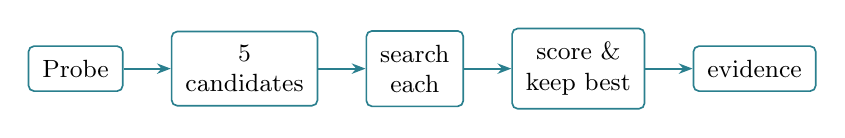
\begin{tikzpicture}[node distance=6mm]
    \node[lp] (p) {Probe};
    \node[lp, right=of p] (c) {5\\candidates};
    \node[lp, right=of c] (s) {search\\each};
    \node[lp, right=of s] (k) {score \&\\keep best};
    \node[lp, right=of k] (e) {evidence};
    \draw[fl] (p) -- (c);
    \draw[fl] (c) -- (s);
    \draw[fl] (s) -- (k);
    \draw[fl] (k) -- (e);
  \end{tikzpicture}
  \end{center}
  \vspace{0.9em}
  \begin{itemize}
    \item The score \alert{never sees the answer}: it rewards results near a target
          count and on-topic with the probe, and penalizes \emph{empty},
          \emph{too broad}, and \emph{repeated} queries.
    \item The hard failures were simply \alert{zero-result} queries --- proposing
          several and dropping the empties already recovers \alert{0/72 $\to$ 25/72}.
  \end{itemize}
\end{frame}

% ---------------------------------------------------------------
\section{Takeaways}

\begin{frame}{Takeaways}
  \begin{itemize}
    \item A small memory agent fails \alert{in stages}: contract $\to$ retrieval $\to$ grounding.
          \smallskip
    \item Tool-call control, query policy, and evidence grounding are
          \alert{different problems} --- one teacher trajectory copies all three too coarsely.
          \smallskip
    \item Build and evaluate small memory agents \alert{component by component}.
          \smallskip
    \item Put query-policy diagnostics \alert{before} broad claims about long-term memory.
  \end{itemize}
\end{frame}

% ---------------------------------------------------------------
\begin{frame}[standout]
  Thank you
  \vspace{0.6em}

  {\small\normalfont jeff4380@unist.ac.kr}
\end{frame}

\end{document}
